% =====================================================================
% Supplementary Information
% =====================================================================
\documentclass[11pt,a4paper]{article}

\usepackage[margin=1in]{geometry}
\usepackage[utf8]{inputenc}
\usepackage[T1]{fontenc}
\usepackage{amsmath,amssymb}
\usepackage{graphicx}
\usepackage{booktabs}
\usepackage{natbib}
\usepackage{hyperref}

\renewcommand{\thefigure}{S\arabic{figure}}
\renewcommand{\thetable}{S\arabic{table}}
\renewcommand{\theequation}{S\arabic{equation}}
\renewcommand{\thesection}{S\arabic{section}}

\newcommand{\sfsix}{SF$_6$}
\newcommand{\kdiss}{k_{\mathrm{diss}}}
\newcommand{\nel}{n_e}

\graphicspath{{../paper/figures/}}

\title{Supplementary Information for\\
       ``What two etch-rate measurements constrain:
       identifiability and EEDF sensitivity of a reduced \sfsix{}
       ICP model''}
\author{[Author list]}
\date{\today}

\begin{document}
\maketitle

\section{Reproducibility}
\label{sec:SI-repro}

All numerical values in the main text and in this supplement
reproduce from a single run of
\texttt{code/main\_reproduction\_script.py} in the project
repository. The script reads the fixed kinetics data (Biagi \sfsix{}
cross sections aggregated via BOLSIG$^+$), executes the two-stage
calibration against the \citet{mansano1999} and \citet{panduranga2019}
anchors under both Maxwellian and two-term Boltzmann rate sources,
and writes the summary CSV to
\texttt{data/processed/m7g\_sweep\_comparison.csv}. Figure
regeneration is handled by \texttt{code/generate\_figures.py} and
writes PDF/PNG files at 300\,dpi to
\texttt{outputs/figures\_300dpi/}.

A verification harness is included as a consistency check. A
reader who runs the pipeline against the committed kinetics table
and does \emph{not} reproduce the values in Table~S\ref{tab:SI-numbers}
to within $10^{-3}$ relative tolerance should open an issue against
the repository before trusting any downstream conclusion.

\begin{table}[h]
  \centering
  \caption{Key numerical values from the calibration pipeline. All
  values reproduce from a single run of the reproduction script.}
  \label{tab:SI-numbers}
  \small
  \begin{tabular}{lll}
    \toprule
    Quantity & Maxwellian & Two-term Boltzmann \\
    \midrule
    Fitted $\beta$ (ms)                & $14.27$       & $509.22$ \\
    Fitted $\varepsilon$ (m\,atom$^{-1}$)
                                       & $7.73\times 10^{-30}$
                                       & $2.76\times 10^{-28}$ \\
    $\kdiss(100\,\mathrm{Td})$ (m$^3$\,s$^{-1}$)
                                       & $1.109\times 10^{-17}$
                                       & $3.804\times 10^{-19}$ \\
    $\nel(P_H = 2\,\mathrm{kW})$ (m$^{-3}$)
                                       & $1.574\times 10^{19}$
                                       & $1.285\times 10^{19}$ \\
    Invariant $\beta\,\kdiss\,\nel(P_H)$
                                       & $2.491$       & $2.487$ \\
    Anchor reproduction: $r(200\,\mathrm{W})$ (nm\,min$^{-1}$)
                                       & $1400.00$     & $1400.00$ \\
    Anchor reproduction: $r(2000\,\mathrm{W})$ (nm\,min$^{-1}$)
                                       & $2270.00$     & $2270.00$ \\
    \bottomrule
  \end{tabular}
\end{table}

\section{Isothermal closed-form verification}
\label{sec:SI-isothermal}

The closed-form isothermal prediction from equation (8) of the
main text gives
$\beta\alpha = 6.7414\times 10^{-3}\,\mathrm{W}^{-1}$ which, with
the isothermal value of
$\alpha = \kdiss/(n_{\mathrm{SF}_6,0}V\,\varepsilon_{\mathrm{loss}}q_e)$,
corresponds to $\beta_{\mathrm{iso}}^{\mathrm{pred}} = 77.27\,$ms.
A direct numerical fit with $\alpha_T = 0$ returns
$\beta_{\mathrm{iso}} = 77.26\,$ms, in agreement to $0.02\,\%$.
Table~S\ref{tab:SI-scaling} reports the artificial $\kdiss$
rescaling test in the isothermal limit that confirms the linearity
of the invariant.

\begin{table}[h]
  \centering
  \caption{Artificial $\kdiss$ rescaling test (isothermal). The
  product $f\cdot\beta_{\mathrm{fit}}$ is constant to numerical
  tolerance, confirming the identifiability theorem.}
  \label{tab:SI-scaling}
  \begin{tabular}{cccc}
    \toprule
    $f$     & $\beta_{\mathrm{fit}}$ (ms)
            & $f\cdot\beta_{\mathrm{fit}}$ (ms)
            & predicted slope \\
    \midrule
    $1.00$  & $77.27$   & $77.27$ & --- \\
    $0.50$  & $154.53$  & $77.27$ & $1.000$ \\
    $0.30$  & $257.57$  & $77.27$ & $1.000$ \\
    $0.10$  & $772.70$  & $77.27$ & $1.000$ \\
    \bottomrule
  \end{tabular}
\end{table}

\section{Non-uniformity comparison}
\label{sec:SI-nu}

Figure~S\ref{fig:nu} shows the wafer-edge-to-center
non-uniformity predicted by both the Maxwellian-calibrated and
Boltzmann-calibrated models as a function of absorbed power. The
two curves are identical to within the tolerance of the numerical
PDE solve, which is a corollary of the identifiability theorem of
the main text: the depletion correction enters the source term as
a scalar prefactor that cancels from the uniformity ratio, and the
non-uniformity is set entirely by the temperature-dependent
diffusion coefficient and the Robin wall boundary condition.

\begin{figure}[h]
  \centering
  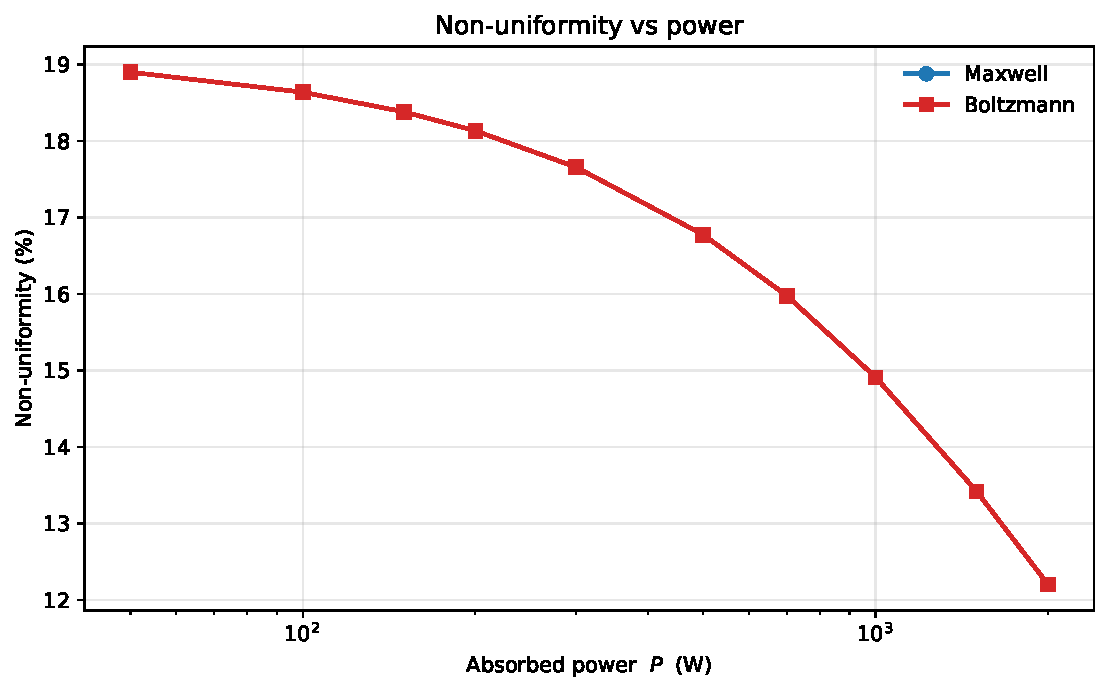
\includegraphics[width=0.62\linewidth]{fig4_nu_comparison}
  \caption{Wafer non-uniformity versus absorbed power for both rate
  sources. The two calibrated models give identical uniformity
  predictions at every power, confirming that the fitted
  depletion parameter has no influence on the non-uniformity
  observable.}
  \label{fig:nu}
\end{figure}

\section{Observability diagnostic data}
\label{sec:SI-obs}

The observability sweep of \S6 of the main text was generated by
holding both calibrated pipelines fixed and evaluating the etch
rate at a regular grid of $(E/N, x_{\mathrm{Ar}}, P)$ operating
points. The grid resolution was $5\,$Td in $E/N$ over
$[50,300]\,$Td, $0.05$ in $x_{\mathrm{Ar}}$ over $[0, 0.75]$,
and three absorbed-power values $(50, 200, 1000)\,$W. The raw
diagnostic data are provided at
\texttt{data/processed/m7g\_observability\_sweep.csv} in the
repository.

\section{Kinetics provenance}
\label{sec:SI-kinetics}

The Maxwellian and two-term Boltzmann rate-coefficient tables
used throughout this work are both aggregated from the same Biagi
\sfsix{} and Ar cross-section sets retrieved from LXCat on
$2026\text{-}04\text{-}14$ \citep{biagi}. Both aggregates use
the same set of channel labels:
\begin{itemize}\small
  \item Ionization: all
        $\mathrm{SF}_6 \to \mathrm{SF}_n^+$ channels,
  \item Attachment: all
        $\mathrm{SF}_6 + e^- \to \mathrm{SF}_n^-$ channels,
  \item Dissociation: all 25 singlet and triplet dissociative
        excitation channels plus the ion-pair excitation channel
        that produces a free \textrm{F} atom.
\end{itemize}
The BOLSIG$^+$ solution \citep{hagelaar2005} was run on the same
$(E/N, x_{\mathrm{Ar}})$ grid as the Maxwellian convolution so
that the comparison of the two rate sources is rigorously
apples-to-apples.

\bibliographystyle{plainnat}
\bibliography{../paper/references}

\end{document}
